\chapter{Resultados}
\label{ch:06}

% \epigraph{\itshape Those who cannot remember the past are condemned to compute it.''}{---Steven Pinker, \textit{Words and Rules}}
% “Language, never forget, is more fashion than science, and matters of usage, spelling and pronunciation tend to wander around like hemlines.” 
% ― Bill Bryson, The Mother Tongue: English and How It Got That Way

% Neste capítulo serão discutidos resultados de múltiplos experimentos realizados a partir de diferentes tipos de modelagem de redes neurais. A primeira delas, baseada na pesquisa de Rumelhart e McClelland, discutida na Seção \ref{sec:arqFDD} e nomeada de FFD.
% A segunda, o modelo de Encoder-Decoder discutido na Seção \ref{sec:enc-dec}. Todos os resultados obtidos a partir dos treinamentos estão organizados e disponíveis em: 
% \url{https://github.com/beatrizalbiero/MsResearch} nas seções \textbf{Wickelfeatures Net Results} e \textbf{Encoder-Decoder}.


% \section{Corpus}
% \label{sec:corpus-ffd}

% Para a execução dos experimentos, foi necessário restringir o escopo da pesquisa a um único tempo, modo, pessoa e número, já que o português apresenta formas irregulares em múltiplas combinações destes elementos e seria necessário construir uma rede diferente para cada uma destas combinações. Optou-se por estudar as irregularidades presentes nas flexões de primeira pessoa do singular no tempo presente, modo indicativo.  
% O corpus utilizado para o treinamento dessa rede foi baseado nas informações contidas em \url{https://www.conjugacao.com.br/verbos-irregulares/} e \url{https://www.conjugacao.com.br/verbos-regulares/}.\\

% Primeiramente, foi realizada uma etapa de extração dos verbos e suas respectivas conjugações para um banco de dados local via técnica de \textit{webscraping}, uma técnica que extrai informações contidas nas páginas da web. Em seguida, os verbos irregulares foram selecionados manualmente para diferentes famílias. Alguns dos verbos irregulares listados nas fontes não eram irregulares no processo de interesse e portanto foram realocados para o grupo de verbos regulares. Como um exemplo disto, um dos motivos para o verbo \textit{acudir} ser considerado irregular é a flexão que ocorre na terceira pessoa do singular no tempo presente e modo indicativo (acode), porém como na primeira pessoa do singular o padrão regular se mantém, esse verbo foi realocado para o grupo dos verbos regulares. Em seguida, os verbos foram transcritos manualmente para uma forma fonológica seguindo a codificação da Tabela \ref{tab:Tab1}. Dos 423 verbos extraídos, 20 foram considerados verbos sem possível agrupamento (verbos como "ir", "trazer" e "saber"), totalizando uma base de 214 verbos regulares e 209 regulares (50.6\% e 49.4\% respectivamente). A Tabela \ref{tab:classes} associa os nomes dados aos tipos de irregularidades encontradas e apresenta um exemplo de cada uma delas. 

% Em seguida, a base foi segmentada entre treino ($\thicksim$80\%) e teste ($\thicksim$20\%) respeitando-se as proporções intra-classe. As Tabelas \ref{tab:g1} e \ref{tab:g3} resumem o número de exemplos presentes nas bases de treino e teste de cada respectiva classe. A Tabela \ref{tab:ratios} exibe as quantidades e proporções finais utilizadas nas bases de treino e teste.


% \begin{table}[H]
% \begin{center}
% \begin{tabular}{l}
% Classes\\
% \toprule
% o\_ar:O\_u $\rightarrow$ tocar, toco\\
% o\_ir:u\_o $\rightarrow$ cobrir, cubro\\
% izer:igu $\rightarrow$ dizer, digo\\
% fazer:fasu $\rightarrow$ fazer, faço\\
% crer:eiu $\rightarrow$ crer, creio\\
% entir:intu $\rightarrow$ sentir, sinto\\
% or:oniu $\rightarrow$ pôr, ponho\\
% e\_ir:i\_u $\rightarrow$ seguir, sigo\\
% ter:teniu $\rightarrow$ ter, tenho\\
% e\_ar:E\_u $\rightarrow$ testar, testo\\
% ver:veju $\rightarrow$ ver, vejo\\
% vir:veniu $\rightarrow$ vir, venho
% \end{tabular}
% \end{center}
% \captionof{table}{Classes de Verbos Irregulares}
% \label{tab:classes}
% \end{table}


% \begin{table}[H]
% \begin{center}
% \begin{tabular}{llllllll}
% iar: eiu & o\_ar: O\_u & o\_ir: u\_o & izer: igu & fazer: fasu & ler, crer: eiu & entir: intu & edir: Esu \\
% 7        & 24          & 6           & 6         & 12          & 4              & 6           & 6\\
% \midrule
% or: oniu & e\_ir: i\_u & ter: teniu & e\_ar: E\_u & ver: veju & vir: veniu & regulares & \\
% 22       & 22          & 8          & 16          & 5         & 8          & 172  &
% \end{tabular}
% \end{center}
% \captionof{table}{Quantidades de Verbos por Classe no Treino}
% \label{tab:g1}
% \end{table}

% \begin{table}[H]
% \begin{center}
% \begin{tabular}{llllllll}
% iar: eiu & o\_ar: O\_u & o\_ir: u\_o & izer: igu & fazer: fasu & ler, crer: eiu & entir: intu & edir: Esu \\
% \toprule
% 2        & 6          & 1           & 1        & 3         & 1              & 2          & 1 \\
% \midrule
% or: oniu & e\_ir: i\_u & ter: teniu & e\_ar: E\_u & ver: veju & vir: veniu & regulares \\

% 5        & 5           & 2          & 4           & 1         & 2          & 42      
% \end{tabular}
% \end{center}
% \captionof{table}{Quantidades de Verbos por Classe no Teste}
% \label{tab:g3}
% \end{table}


% \begin{table}[H]
% \begin{center}
% \begin{tabular}{lllll}
% \hline
%  & \textbf{Regulares} & \textbf{Irregulares} & \textbf{Total} & \textbf{\%} \\ \hline
% \textbf{Teste} & 42 & 36 & 78 & 19.35 \\ \hline
% \textbf{Treino} & 172 & 153 & 325 & 80.65 \\ \hline
% \textbf{Total} & 214 & 189 & 403 & 100 \\ \hline
% \end{tabular}
% \end{center}
% \captionof{table}{Proporção entre Verbos Regulares e Irregulares nos datasets}
% \label{tab:ratios}
% \end{table}


% \section{Rede FFD}
% \label{sec:ffd}

% A rede desenvolvida possui uma camada de Input (Verbos no Infinitivo) e uma de Output (Verbos Flexionados), ambas compostas por 460 unidades, cada unidade representando um Wickelfeature. Para a construção da rede, foi utilizada a linguagem de programação \textit{Python} e a biblioteca \textit{Keras} (\cite{chollet2015keras}).

% \subsection{Hiperparâmetros}

% Em redes neurais, existem os parâmetros que são atualizados em decorrência do treinamento (os pesos, por exemplo) e existem parâmetros que devem ser escolhidos antes do treinamento e permanecem fixos. Esse segundo tipo de parâmetro é considerado um \textit{hiperparâmetro}. A escolha dos melhores hiperparâmetros de um modelo de redes neurais é totalmente experimental e envolve uma série de estratégias. Muitas vezes os hiperparâmetros são escolhidos a partir de indicações na literatura. Caso o acesso a tais referências seja limitado por qualquer razão, faz-se necessária a realização de uma série de experimentos a fim de se testar diferentes possibilidades e combinações de hiperparâmetros. Ainda há uma terceira estratégia que é a utilização de algoritmos de busca (Grid Search\footnote{\cite{Goodfellow-et-al-2016}, Cap. 6}, por exemplo). Esta pesquisa utilizou-se da primeira e segunda estratégia até o presente momento para a demonstração dos resultados. Alguns dos hiperparâmetros mais importantes são: a função de custo, a função de ativação e o número de épocas. A primeira coisa a ser definida é a função de custo. O aprendizado de uma rede neural ocorre principalmente em decorrência da comparação entre os valores preditos e os valores desejados. Tal diferença pode ser calculada a partir de uma medida de distância entre esses valores. Nesta pesquisa foi utilizada a função de erros quadráticos médios, que é uma função adequada para o tipo de problema apresentado. Em seguida, é preciso escolher uma função de ativação. A função de ativação escolhida foi a \textit{Sigmoid} por se tratar da mesma função utilizada pelos pesquisadores Rumelhart e McClelland. Por último, é preciso escolher o número de \textit{Épocas} do treinamento. O número de épocas se refere à quantidade de vezes em que os exemplos passam passam pela rede. Um número de épocas pequeno pode ser insuficiente para o aprendizado e um número de épocas grande pode causar um fenômeno chamado de \textit{overfitting}, aonde a rede adquire um bom desempenho nos exemplos de treinamento porém é incapaz de obter o mesmo desempenho em exemplos novos. Após alguns experimentos com diferentes números, percebeu-se que em até 400 épocas, o modelo apresentava bons resultados e que, a partir desse valor, o aprendizado da rede ficava estagnado.

% \begin{table}[H]
% \centering
% \begin{tabular}{ll}
% Custo: & erro quadrático médio \\
% Ativação: & sigmoid \\
% Épocas: & 400 \\
% \end{tabular}
% \caption{Tabela Resumo dos Hiperparâmetros do Modelo FFD}
% \label{tab:resumo1}
% \end{table}

% \subsection{Resultados}

% O modelo FFD foi treinado em diferentes bases com diferentes arranjos proporcionais de verbos irregulares contra regulares. Esses testes foram realizados com o intuito de testar se a frequência de verbos irregulares pode influenciar no processo de aprendizado dos mesmos. Todos os modelos foram testados em 21 verbos, sendo 16 destes irregulares. A base de teste foi escolhida de modo a testar o modelo em famílias irregulares diversas. Para a avaliação dos modelos foi considerada a métrica de acurácia, ou seja, a proporção de acertos nos testes. 

% \begin{equation}
% Acurácia = \frac{Acertos}{Total}
% \end{equation}

% A Tabela \ref{tab:resultadosfdd} resume os resultados obtidos a serem discutidos na Seção \ref{sec:disc}.

% \begin{table}[H]
% \centering
% \begin{tabular}{llllll}
%  & \textbf{55\%} & \textbf{65\%} & \textbf{75\%} & \textbf{85\%} & \textbf{95\%} \\ \hline
% \textbf{Acurácia} & 47.62\% & 38.10\% & 38.10\% & 42.86\% & 47.62\% 
% \end{tabular}
% \caption{Resultados para diferentes proporções de verbos irregulares na base de treino para a rede FDD.}
% \label{tab:resultadosfdd}
% \end{table}

% O modelo falhou na decodificação de Wickelfeatures em 7 casos, justamente em verbos com sequências maiores de fonemas. Também é importante notar que entre estes, 6 casos foram observados em que o modelo foi capaz de prever o processo de inflexão irregular apesar de falhar em decodificar os fonemas centrais das palavras, são os casos dos verbos \textit{postar, mentir, compor, por, sortear e mediar}. Esses casos foram contabilizados na contagem da acurácia.

% \begin{table}[H]
% \centering
% \begin{tabular}{llll}
% \textbf{Verbo} & \textbf{Input} & \textbf{Esperado} & \textbf{Output} \\ \hline
% pegar & \#pega\# & \#pEgu\# & \#pEku\# \\
% cegar & \#sega\# & \#sEgu\# & \#sigu\# \\
% secar & \#seka\# & \#sEku\# & \#siku\# \\
% levar & \#leva\# & \#lEvu\# & \#levu\# \\
% orar & \#ora\# & \#Oru\# & \#earu\# \\
% morar & \#mora\# & \#mOru\# & \#mEru\# \\
% postar & \#posta\# & \#pOstu\# & \#pOtu\#* \\
% mentir & \#menti\# & \#mintu\# & \#mitu\#* \\
% jogar & \#joga\# & \#jOgu\# & \#xogu\# \\
% compôr & \#kompo\# & \#komponiu\# & \#koiu\#*\\
% pôr & \#po\# & \#poniu\# & \#poiu\#*\\
% sortear & \#sortia\# & \#sorteiu\# & \#soiu\#*\\
% mediar & \#media\# & \#medeiu\# & \#meiu\#*\\
% cobrir & \#kobri\# & \#kubro\# & \#koru\#\\
% tossir & \#tosi\# & \#tusu\# & \#tutu\# \\
% fazer & \#faze\# & \#fasu\# & \#fasu\# \\
% matar & \#mata\# & \#matu\# & \#matu\# \\
% pagar & \#paga\# & \#pagu\# & \#pagu\# \\
% bater & \#bate\# & \#batu\# & \#baiu\# \\
% sair & \#sai\# & \#saiu\# & \#saiu\#\\
% comer & \#kome\# & \#komu\# & \#koiu\#\\
% \end{tabular}
% \caption{Resultados Modelo FFD com Proporção de 95\% de Verbos Irregulares no Treinamento}
% \label{tab:res}
% \end{table}

\section{Introdução}
\label{sec:seq2seq}

% Como discutido na Seção \ref{sec:enc-dec}, os modelos do tipo Encoder-Decoder parecem promissores para que se possa alcançar os objetivos propostos dada a dificuldade encontrada na decodificação de longas sequências. %Nessa seção são discutidos e comparados alguns testes relacionados à mesma arquitetura (Fig. \ref{fig:encdec}), porém alteram-se alguns dos hiperparâmetros possíveis e testam-se também bases de diferentes comprimentos.

A camada de Input do Encoder é inicializada a partir do tamanho do vocabulário. Nesse caso, considera-se vocabulário o número de fonemas únicos contidos na base de treinamento para a forma infinitiva dos verbos. Na camada de Input do Decoder, equivalentemente, o vocabulário da forma verbal flexionada.
%incluir ref Keras

Os outputs da rede Encoder são descartados e seus estados finais inicializam os pesos da rede Decoder. Por último, os outputs da rede Decoder passam por uma camada densa (sem recorrência, assim como a FFD).

A Fig.\ref{fig:encdec} foi construída utilizando a biblioteca \textit{Keras} para ilustrar um resumo da arquitetura do Encoder-Decoder.

\begin{figure}[H]
  \centering
  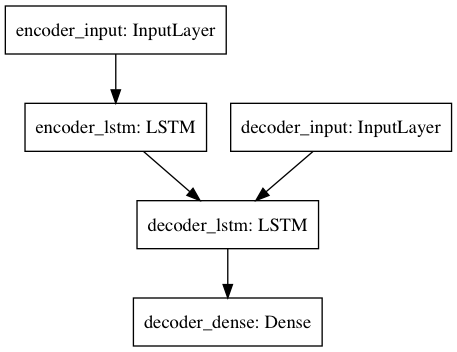
\includegraphics[width=0.5\linewidth]{img/draw-model6.png}
  \caption{Arquitetura Encoder-Decoder Desenvolvida}
  \label{fig:encdec}
\end{figure}

Assim como na rede FFD, foi utilizada a linguagem de programação \textit{Python} e a biblioteca \textit{Keras}.

\section{Apresentação}

% mudar essa seção daqui pra cima\subsubsection{Corpus}
% O modelo \textbf{Encoder-Decoder} foi treinado na base apresentada na Seção \ref{sec:corpus-ffd}, para o caso de proporção de 55\% de verbos irregulares. Como o sistema de redes neurais recorrentes independe dos indicadores de fronteira (\#), estes foram retirados do pré-processamento dos verbos da base.

% falar sobre hiperparametros mais pra cima\subsubsection{Hiperparâmetros} 

% Os hiperparâmetros deste modelo foram escolhidos com base em uma tarefa similar de tradução automática entre francês e inglês apresentada no tutorial de \cite{tutorial}. No tutorial, Chollet apresenta o desenvolvimento do algoritmo, bem como os hiperparâmetros escolhidos.  

% \begin{table}[H]
% \centering
% \begin{tabular}{ll}
% Custo: & categorical\_crossentropy \\
% Ativação & softmax \\
% Épocas & 150 \\
% \end{tabular}
% \caption{Resumo dos Hiperparâmetros do Modelo Encoder-Decoder 1}
% \label{tab:resumo21}
% \end{table}

% Numero de Amostras Treinamento: & 452 \\
% Numero de Amostras Teste: & 21 \\
% Numero de tokens unicos do Input: & 23 \\
% Numero de tokens unicos do Output: & 27 \\
% Comprimento maximo da sequencia para inputs: & 13 \\
% Comprimento maximo da sequencia para outputs: & 15 \\

%\subsubsection{Resultados}

% \begin{figure}[H]
%   \centering
%   \begin{subfigure}[b]{0.45\linewidth}
%     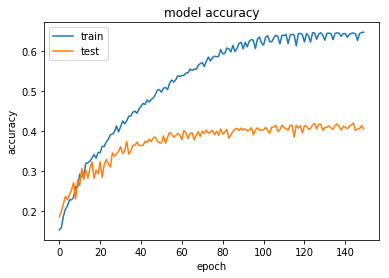
\includegraphics[width=\linewidth]{img/enc-dec-2.png}
%     \caption{Resultados de Acurácia por Época}
%   \end{subfigure}
%   \begin{subfigure}[b]{0.45\linewidth}
%     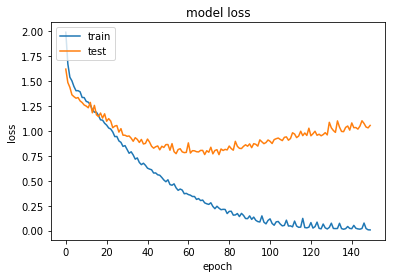
\includegraphics[width=\linewidth]{img/enc-dec-2-loss.png}
%     \caption{Resultados de Custo por Época}
%   \end{subfigure}
%   \caption{Gráficos dos Resultados do Modelo}
%   \label{fig:plots2}
% \end{figure}

% \begin{table}[H]
% \centering
% \begin{tabular}{llllll}
% \textbf{Best Epoch Score} & \textbf{Val\_Acc} & \textbf{Val\_Loss} & \textbf{Loss} & \textbf{Acc} & \textbf{Time} \\
% 145 & 0.419 & 1.048 & 0.014 & 0.644 & 4 min
% \end{tabular}
% \caption{Scores do Modelo Encoder-Decoder 2}
% \label{tab:res-enc-dec-2}
% \end{table}

% \begin{table}[H]
% \centering
% \begin{tabular}{lll}
% \textbf{Input} & \textbf{Expected} & \textbf{Output} \\ \hline
% seka& sEku& sugu \\
% leva& lEvu& levu \\
% ora& Oru& bOtu\\
% mora& mOru& omupu\\
% posta& pOstu& postu\\
% joga& jOgu& ju\\
% sortia& sorteiu& surtu\\
% media& medeiu& medeiu\\
% kompo& komponiu& kompou\\
% po& poniu& poveiniu\\
% menti& mintu& mintu\\
% tosi& tusu& surteiu\\
% \end{tabular}
% \caption{Resultados do modelo Encoder-Decoder}
% \label{tab:res2}
% \end{table}

% O modelo \textbf{Encoder-Decoder} apresentou uma acurácia muito baixa, acertou apenas 2 verbos entre 12. Por outro lado, os 2 verbos que acertou são verbos que a rede FFD seria incapaz de decodificar dado o tamanho das sequências (\textit{mentir} e \textit{mediar}). Além disso regularizou os verbos \textit{levar} e \textit{postar}. Em outros exemplos a rede devolveu verbos flexionados existentes, porém que não diziam respeito ao verbo do \textit{input}. Foi o caso dos verbos \textit{orar}, \textit{sortear} e \textit{tossir}. Isso possivelmente ocorreu em decorrência de uma número reduzido de exemplos similares no treinamento. Como o grau de resolução foi reduzido ao nível dos fonemas, a rede fica extremamente dependente desses exemplos. No caso do verbo \textit{orar}, provavelmente ela foi apresentada durante o treinamento a nenhum exemplo de verbo que começa com o fonema "\textit{o}"  o que resultou na predição de um fonema mais provável (nesse caso o \textit{b}) e a partir de então o restante da predição se deu de acordo com uma sequência iniciando com este fonema e que estava no treinamento, \textit{botar}. Isto também explica o motivo da rede ter acertado os verbos \textit{mentir} e \textit{mediar} pois na base de treinamento haviam verbos como \textit{desmentir} e \textit{remediar}.

% \subsection{Modelo Encoder-Decoder 2} 

% \subsubsection{Corpus}
% O modelo \textbf{Encoder-Decoder 1} foi treinado na base apresentada na Seção \ref{sec:corpus-ffd}, porém sem qualquer balanceamento relativo à proporção de verbos irregulares.

% \subsubsection{Hiperparâmetros} 

% \begin{table}[H]
% \centering
% \begin{tabular}{ll}
% Numero de Amostras Treinamento: & 325 \\
% Numero de Amostras Teste: & 100 \\
% Numero de tokens unicos do Input: & 22 \\
% Numero de tokens unicos do Output: & 26 \\
% Comprimento maximo da sequencia para inputs: & 11 \\
% Comprimento maximo da sequencia para outputs: & 13 \\
% Loss: & categorical\_crossentropy \\
% Optimizer & rmsprop \\
% Activation & softmax \\
% Epochs & 130 \\
% Batch Size & 64
% \end{tabular}
% \caption{Tabela Resumo Estrutural do Modelo Encoder-Decoder 1}
% \label{tab:resumo2}
% \end{table}

% \subsubsection{Resultados}

% \begin{figure}[H]
%   \centering
%   \begin{subfigure}[b]{0.45\linewidth}
%     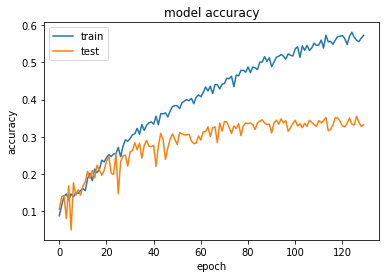
\includegraphics[width=\linewidth]{img/enc-dec-1.png}
%     \caption{Resultados de Acurácia por Época}
%   \end{subfigure}
%   \begin{subfigure}[b]{0.45\linewidth}
%     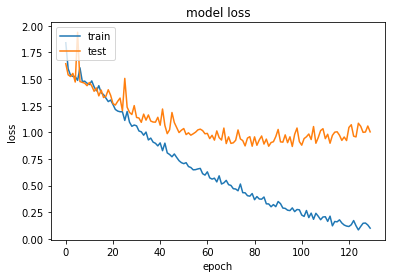
\includegraphics[width=\linewidth]{img/enc-dec-1-loss.png}
%     \caption{Resultados de Custo por Época}
%   \end{subfigure}
%   \caption{Gráficos dos Resultados do Modelo}
%   \label{fig:plots1}
% \end{figure}

% \begin{table}[H]
% \centering
% \begin{tabular}{llllll}
% \textbf{Best Epoch Score} & \textbf{Val\_Acc} & \textbf{Val\_Loss} & \textbf{Loss} & \textbf{Acc} & \textbf{Time} \\
% 97 & 0.342 & 0.867 & 0.290 & 0.508 & 2 min
% \end{tabular}
% \caption{Scores do Modelo Encoder-Decoder 1}
% \label{tab:res-enc-dec-1}
% \end{table}

% \begin{table}[H]
% \centering
% \begin{tabular}{lll}
% \textbf{Input} & \textbf{Expected} & \textbf{Output} \\ \hline
% segir& sigu& siriu\\
% hepeti& hepitu& hespeniu\\
% dete& deteniu& desiru\\
% te& teniu& teniu\\
% protesta& protEstu& proteiu\\
% espera& espEru& esprEsu\\
% pega& pEgu& pEsu\\
% sega& sEgu& sEsu\\
% preve& preveju& previnu\\
% vi& veniu& viju\\
% adivi& adiveniu& aiijasu\\
% junta& juntu& jugu\\
% \end{tabular}
% \caption{Alguns resultados interessantes do modelo Encoder-Decoder 1}
% \label{tab:res1}
% \end{table}

% O modelo \textbf{Encoder-Decoder 1} apesar de ter mais facilidade na predição de sequências longas apresentou resultados inferiores ao modelo \textbf{FFD}. A Tabela \ref{tab:res1} exibe uma série de predições que seriam consideradas sem nexo para falantes. Apesar disso, é possível notar que a rede foi capaz de relacionar alguns verbos do teste com suas respectivas famílias irregulares. Os verbos 'pegar' e 'esperar' por exemplo foram associados corretamente às suas respectivas famílias apesar de terem sido conjugados de forma equivocada.


% \subsection{Modelo Encoder-Decoder 3}
 
% \subsubsection{Corpus e Metodologia}

% O corpus utilizado para o treinamento das redes \textbf{Encoder-Decoder 3}, \textbf{Encoder-Decoder 4} e \textbf{Encoder-Decoder 5}  foi baseado na lista de verbos disponíveis no site \url{https://www.conjugacao.com.br/verbos-populares/}.\\

% As informações contidas nessa página diferem-se das páginas apresentadas na Seção \ref{sec:corpus-ffd} no sentido de que, em primeiro lugar, não há qualquer divisão entre verbos regulares ou irregulares (o que dificulta a segmentação manual dos verbos em diferentes famílias); apesar disso, ganha-se ao aumentar em quase cem vezes o tamanho da base de treino. 

% Assim como na Seção \ref{sec:corpus-ffd}, foi realizada uma etapa de extração dos verbos e suas respectivas conjugações para um banco de dados local. Em seguida, os verbos foram mantidos em notação ortográfica como um exercício de prova de conceito. O objetivo dos testes que se seguem é avaliar o potencial preditivo quando se pode contar com uma base de treinamento consideravelmente maior. Perde-se pela considerável redução de resolução com relação ao reconhecimento de padrões fonológicos, fato que será discutido na Seção \ref{sec:disc}

% \subsubsection{Hiperparâmetros} 

% \begin{table}[H]
% \centering
% \begin{tabular}{ll}
% Numero de Amostras Treinamento: & 2000 \\
% Numero de Amostras Teste: & 100 \\
% Numero de tokens unicos do Input: & 26 \\
% Numero de tokens unicos do Output: & 32 \\
% Comprimento maximo da sequencia para inputs: & 15 \\
% Comprimento maximo da sequencia para outputs: & 16 \\
% Loss: & categorical\_crossentropy \\
% Optimizer & rmsprop \\
% Activation & softmax \\
% Epochs & 100 \\
% Batch Size & 64
% \end{tabular}
% \caption{Tabela Resumo Estrutural do Modelo Encoder-Decoder 3}
% \label{tab:resumo3}
% \end{table}

% \subsubsection{Resultados}
% %falar q eu adicionei dropout e explicar oq é isso

% \begin{figure}[H]
%   \centering
%   \begin{subfigure}[b]{0.45\linewidth}
%     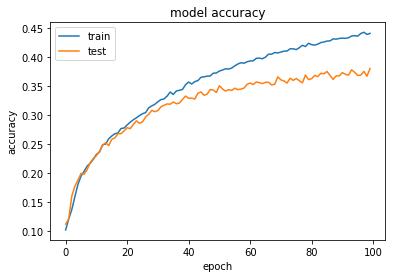
\includegraphics[width=\linewidth]{img/enc-dec-3.png}
%     \caption{Resultados de Acurácia por Época}
%   \end{subfigure}
%   \begin{subfigure}[b]{0.45\linewidth}
%     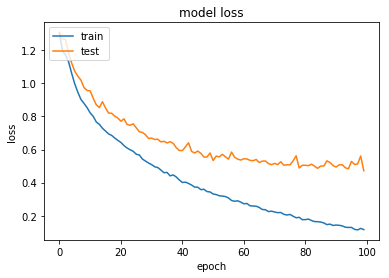
\includegraphics[width=\linewidth]{img/enc-dec-3-loss.png}
%     \caption{Resultados de Custo por Época}
%   \end{subfigure}
%   \caption{Gráficos dos Resultados do Modelo}
%   \label{fig:plots3}
% \end{figure}

% \begin{table}[H]
% \centering
% \begin{tabular}{llllll}
% \textbf{Best Epoch Score} & \textbf{Val\_Acc} & \textbf{Val\_Loss} & \textbf{Loss} & \textbf{Acc} & \textbf{Time} \\
% 100 & 0.380 & 0.471 & 0.115 & 0.440 & 11 min
% \end{tabular}
% \caption{Scores do Modelo Encoder-Decoder 3}
% \label{tab:res-enc-dec-3}
% \end{table}

% \begin{table}[H]
% \centering
% \begin{tabular}{lll}
% \textbf{Input} & \textbf{Expected} & \textbf{Output} \\ \hline
% salgar& salgo& salgo\\
% barrar& barro& barro\\
% inquirir& inquiro& inquiro\\
% empobrecer& empobreço& empolero\\
% abreviar& abrevio& abrivejo\\
% folhar& folho& folheio\\
% repudiar& repudio& repudo\\
% desabafar& desabafo& desabaco\\
% estampar& estampo& estamo\\
% filtrar& filtro& filtro\\
% migrar& migro& migro\\
% pilar& pilo& pilo\\
% bolar& bolo& bolo\\
% voltear& volteio& volteio\\
% explicitar& explicito& explico
% \end{tabular}
% \caption{Alguns resultados interessantes do modelo Encoder-Decoder 3}
% \label{tab:res3}
% \end{table}

% Nesse modelo foi acrescentada uma técnica de regularização conhecida como Dropout. Essa técnica consiste na inativação aleatória de algumas unidades durante o treinamento para previnir o efeito de overfitting. O modelo de \textbf{Encoder-Decoder 3} exibe previsões mais interessantes que os modelos anteriores. Muitas das predições erraram por apenas uma edição de caracter, mas ainda são erros que falantes provavelmente não cometeriam. No entanto, é natural que a rede perca resolução dado que o nível de treinamento foi alterado de traços fonológicos para caracteres.

% \subsection{Modelo Encoder-Decoder 4}
% %Falar que eu quis mudar a funcao de ativacao pra ver oq acontecia e o otimizador tb (deve ter tido uma razao pra eu ter feito isso, deve ta no deep learning la)

% \subsubsection{Hiperparâmetros} 

% \begin{table}[H]
% \centering
% \begin{tabular}{ll}
% Numero de Amostras Treinamento: & 2000 \\
% Numero de Amostras Teste: & 100 \\
% Numero de tokens unicos do Input: & 26 \\
% Numero de tokens unicos do Output: & 29 \\
% Comprimento maximo da sequencia para inputs: & 15 \\
% Comprimento maximo da sequencia para outputs: & 16 \\
% Loss: & categorical\_crossentropy \\
% Optimizer & adam \\
% Activation & relu \\
% Epochs & 100 \\
% Batch Size & 64
% \end{tabular}
% \caption{Tabela Resumo Estrutural do Modelo Encoder-Decoder 4}
% \label{tab:resumo4}
% \end{table}

% \subsubsection{Resultados}

% \begin{figure}[H]
%   \centering
%   \begin{subfigure}[b]{0.45\linewidth}
%     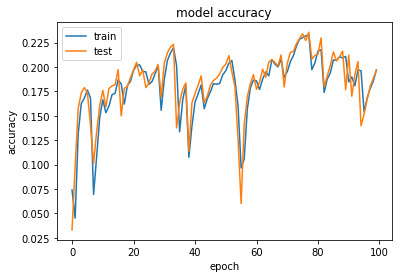
\includegraphics[width=\linewidth]{img/enc-dec-4.png}
%     \caption{Resultados de Acurácia por Época}
%   \end{subfigure}
%   \begin{subfigure}[b]{0.45\linewidth}
%     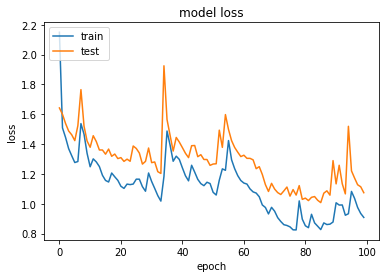
\includegraphics[width=\linewidth]{img/enc-dec-4-loss.png}
%     \caption{Resultados de Custo por Época}
%   \end{subfigure}
%   \caption{Gráficos dos Resultados do Modelo}
%   \label{fig:plots4}
% \end{figure}

% \begin{table}[H]
% \centering
% \begin{tabular}{llllll}
% \textbf{Best Epoch Score} & \textbf{Val\_Acc} & \textbf{Val\_Loss} & \textbf{Loss} & \textbf{Acc} & \textbf{Time} \\
% 86 & 0.210 & 1.00 & 0.820 & 0.207 & 10 min
% \end{tabular}
% \caption{Scores do Modelo Encoder-Decoder 4}
% \label{tab:res-enc-dec-4}
% \end{table}

% \begin{table}[H]
% \centering
% \begin{tabular}{lll}
% \textbf{Input} & \textbf{Expected} & \textbf{Output} \\ \hline
% raptar& rapto& aso\\
% salgar& salgo& aulo\\
% barrar& barro& aco\\
% urinar& urino& auso\\
% inquirir& inquiro& eino\\
% folhar& folho& o\\
% refutar& refuto& o\\
% cogitar& cogito& aco\\
% \end{tabular}
% \caption{Alguns resultados interessantes do modelo Encoder-Decoder 4}
% \label{tab:res4}
% \end{table}

% A alteração da função de ativação da rede não surtiu efeitos muito interessantes. Aparentemente isso tornou os resultados mais arbitrários. Além disso, provavelmente reforçou demasiadamente a probabilidade de um token de final de palavra após o fonema \textbf{o}.
 
%  \subsection{Modelo Encoder-Decoder 5}
% %Falar que eu quis aumentar mais ainda a amostra

% \subsubsection{Hiperparâmetros} 

% \begin{table}[H]
% \centering
% \begin{tabular}{ll}
% Numero de Amostras Treinamento: & 3000 \\
% Numero de Amostras Teste: & 100 \\
% Numero de tokens unicos do Input: & 26 \\
% Numero de tokens unicos do Output: & 32 \\
% Comprimento maximo da sequencia para inputs: & 15 \\
% Comprimento maximo da sequencia para outputs: & 16 \\
% Loss: & categorical\_crossentropy \\
% Optimizer & rmsprop \\
% Activation & softmax \\
% Epochs & 100 \\
% Batch Size & 64
% \end{tabular}
% \caption{Tabela Resumo Estrutural do Modelo Encoder-Decoder 5}
% \label{tab:res5}
% \end{table}

% \subsubsection{Resultados}

% \begin{figure}[H]
%   \centering
%   \begin{subfigure}[b]{0.45\linewidth}
%     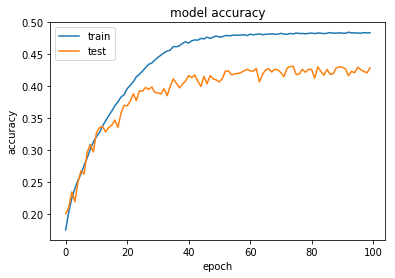
\includegraphics[width=\linewidth]{img/enc-dec-5.png}
%     \caption{Resultados de Acurácia por Época}
%   \end{subfigure}
%   \begin{subfigure}[b]{0.45\linewidth}
%     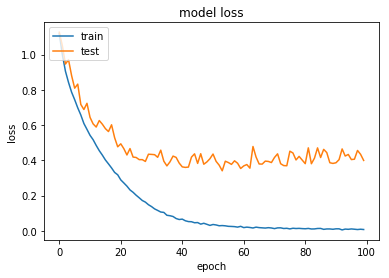
\includegraphics[width=\linewidth]{img/enc-dec-5-loss.png}
%     \caption{Resultados de Custo por Época}
%   \end{subfigure}
%   \caption{Gráficos dos Resultados do Modelo}
%   \label{fig:plots5}
% \end{figure}

% \begin{table}[H]
% \centering
% \begin{tabular}{llllll}
% \textbf{Best Epoch Score} & \textbf{Val\_Acc} & \textbf{Val\_Loss} & \textbf{Loss} & \textbf{Acc} & \textbf{Time} \\
% 54 & 0.423 & 0.340 & 0.030 & 0.4789 & 15 min
% \end{tabular}
% \caption{Scores do Modelo Encoder-Decoder 5}
% \label{tab:res-enc-dec-5}
% \end{table}

% \begin{table}[H]
% \centering
% \begin{tabular}{lll}
% \textbf{Input} & \textbf{Expected} & \textbf{Output} \\ \hline
% enxotar& enxoto& enxoto\\
% expiar& expio& expio\\
% pernear& perneio& perenço\\
% propugnar& propugno& propugo\\
% represar& represo& represo\\
% retaliar& retalio& retalio\\
% taralhar& taralho& taralho\\
% amargar& amargo& amargo\\
% arquear& arqueio& arquejo\\
% desarmonizar& desarmonizo& desmarço\\
% esterilizar& esterilizo& estrialeço\\
% potenciar& potencio& potencio
% \end{tabular}
% \caption{Alguns resultados interessantes do modelo Encoder-Decoder 5}
% \label{tab:resumo5}
% \end{table}

% Aumentar ainda mais a base de treino ainda não produziu uma acurácia muito alta, porém os resultados parecem mais coerentes do que os resultados dos demais modelos. Na Tabela \ref{tab:res5} verificam-se múltiplos exemplos de predições equivocadas em decorrência de uma edição de caracter.

\section{Discussão}
\label{sec:disc}

Na Tabela \ref{tab:resultadosfdd} observa-se que aparentemente não há qualquer relação entre a proporção de verbos irregulares na base de treino e a acurácia do modelo. Apesar da variação percentual ser grande, os modelos podem ser considerados similares pois a base de teste era de apenas 21 verbos e uma predição incorreta de uma única conjugação significa uma perda de 4.76\% na acurácia.\\ 

O modelo Encoder-Decoder foi adotado principalmente pela dificuldade encontrada no processo de decodificação dos verbos para a arquitetura FFD. O cálculo recursivo a nível de fonemas utilizando as RNR's elimina o problema apontado na Seção \ref{sec:dec}. No entanto, como verificado na Tabela \ref{tab:res2} o modelo carece de um número maior de exemplos e portanto apresentou acurácia inferior à arquitetura FFD.\\ 

Para concluir, novos experimentos ainda terão de ser realizados para a construção de uma rede neural capaz de realizar o processo de flexão desejado. É possível que aumentar o espaço amostral de verbos seja suficiente para que o Encoder-Decoder atinja uma acurácia melhor. Por outro lado, também faz-se necessária uma investigação sobre a possibilidade de se aumentar o grau de resolução novamente para o nível de atributos fonológicos e repensar o modelo Encoder-Decoder para que dê conta dessa alteração.

%\textit{1. Aumentar a base de treino parece aprimorar o treinamento de forma razoável}; \textit{2. Aumentar o grau de resolução para transcrição fonética nessa mesma base pode aprimorar o treinamento ainda mais (como observado nos resultados do modelo Encoder-Decoder 2)}; \textit{3. O acréscimo da camada de Dropout surtiu um efeito muito interessante e a combinação com os demais itens apontados pode contribuir ainda mais para o aprimoramento do modelo}.
